\section{TRABALHOS RELACIONADOS}
\label{sec:trabalhos-relacionados}
\citeonline{utfpr2017} propõe em seu trabalho a produção de um recurso educacional para auxiliar o ensino de análise e projeto de \textit{software}. Para suprir a necessidade da prática em matérias de ES, principalmente para os cursos de Engenharia Elétrica, de Computação e Controle e Automação. O recurso educacional proposto consiste em um conjunto de projetos utilizando a plataforma Arduino. Cada projeto possui seis artefatos: o diagrama de casos de uso, o diagrama de atividades, o diagrama de máquinas de estado, o diagrama de classe, o esquemático de montagem e o código fonte em linguagem C/C++. A partir destes artefatos os alunos deveriam analisá-los e embarcá-los na plataforma Arduino, de forma a treinar a capacidade de interpretação de artefatos UML. Os artefatos foram aplicados em 3 turmas do curso de Engenharia de Computação da UTFPR - Câmpus Cornélio Procópio, durante a disciplina de Engenharia de \textit{Software}, onde após a conclusão da utilização, os alunos deram um \textit{feedback} através de um questionário baseado na escala \textit{likert} e uma questão aberta, para possíveis sugestões. As respostas a respeito do recurso educacional foram predominantemente positivas, demonstrando a aceitação pelos alunos e o auxílio no aprendizado.

\citeonline{Garcia2017} apresenta o GOAL, Gamification on Application Lifecycle Management, um \textit{framework} que tem como objetivo a orientação de um processo que suporta a introdução da gamificação em qualquer fase do desenvolvimento de \textit{software}. Um estudo de caso foi realizado pelos autores em uma empresa de desenvolvimento de \textit{software} para investigar a viabilidade de aplicação do \textit{framework} para integrar a gamificação em outros ambientes de engenharia de \textit{software}. Foram gamificadas três áreas de processo utilizando uma metodologia presente no GOAL, as áreas são: gerenciamento de requisitos, gerenciamento de projetos e teste de \textit{software}. Os elementos de jogos escolhidos para a gamificação foram: pontuação, \textit{levels}, distintivos, \textit{leaderboard}, \textit{social graph} e desafios. As conclusões obtidas em relação a utilização do \textit{framework} foram positivas, revelando benefícios oferecidos na utilização do GOAL em um contexto industrial. 

\citeonline{Souza2010} apresenta o SPARSE, um jogo desenvolvido com o intuito de proporcionar a prática no ensino e aprendizagem de ES baseado em jogos e simulação. O jogo visa definir um método de ensino e aprendizado de ES que combine a teoria apresentada em aula com uma abordagem prática, preparando o aluno para cenários reais. O jogo foi apresentado para alunos de Bacharelado em Ciência da Computação de diferentes etapas do curso como método de avaliação para futuras melhorias. Com a análise dos resultados obtidos através de questionários, percebeu-se satisfação da maioria dos jogadores com relação ao uso da ferramenta proposta. Além disso, notou-se um aumento em geral do conhecimento de ES abordado no jogo.

Considerando o potencial da gamificação e poucos estudos no contexto da educação em engenharia de \textit{software}, \citeonline{Borges2014} descreve em seu artigo a experiência da inclusão de dois elementos de jogo, especificamente distintivos e uma tabela de classificação, em um curso introdutório em ES. O objetivo do trabalho é avaliar o entendimento dos alunos em relação ao impacto desses elementos em sua motivação para o curso. Apesar de não utilizar todo o potencial do uso de distintivos, percebeu-se uma grande aceitação, onde eles serviam como uma recompensa social e como um segundo objetivo, além das notas e aprovação. Entretanto, o uso da classificação mostrou opiniões distintas. Os alunos usaram os resultados para comparar seu desempenho em relação aos outros, motivando-se para a obtenção de um melhor desempenho quando tinham notas baixas, porém o foco na utilização das notas para a tabela de classificação foi um aspecto negativo, que poderia ser complementado por outros tipos de medidas.

\chapter{PROPOSTA}
\label{chap:proposta}

Nesta seção são descritas as atividades que serão executadas a fim de atingir os objetivos deste trabalho, bem como as tecnologias utilizadas para o desenvolvimento do mesmo. Esta seção está subdivida em: plicação, ferramentas e utilização da aplicação e \textit{feedback} análise dos resultados.  

\begin{figure}[!htb]
    \centering
    \caption{Diagrama da arquitetura da proposta}
    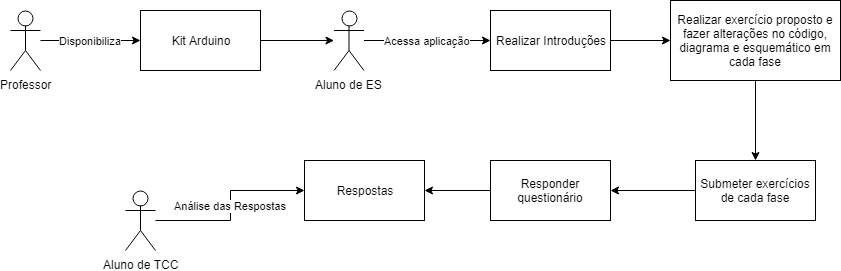
\includegraphics[width=1\textwidth]{./dados/figuras/diagramaProjeto}
    \fonte{Autoria Própria}
    \label{fig:figura-diagramaApp}
\end{figure}

\section{APLICAÇÃO WEB}
\label{sec:desenvApp}



O artefato produzido por este trabalho será uma aplicação web, composta por uma breve introdução sobre a plataforma Arduino e um pequeno projeto a ser desenvolvido, para ambientar os usuários ao cenário. Após isso, será apresentado três áreas de conhecimentos abordadas no projeto, como apresentado na Figura \ref{fig:figura-areas-telas}, onde cada uma será constituída por uma introdução, questionário sobre conceitos e atividades práticas divididas em fases, como visto na Figura \ref{fig:figura-fases-telas}. O avanço em cada fase se dará somente após a resolução do exercício proposto e submissão para correção. A cada fase, o nível de complexidade do projeto será aumentado gradativamente.

\begin{figure}[!htb]
    \centering
    \caption{Áreas de conhecimento}
    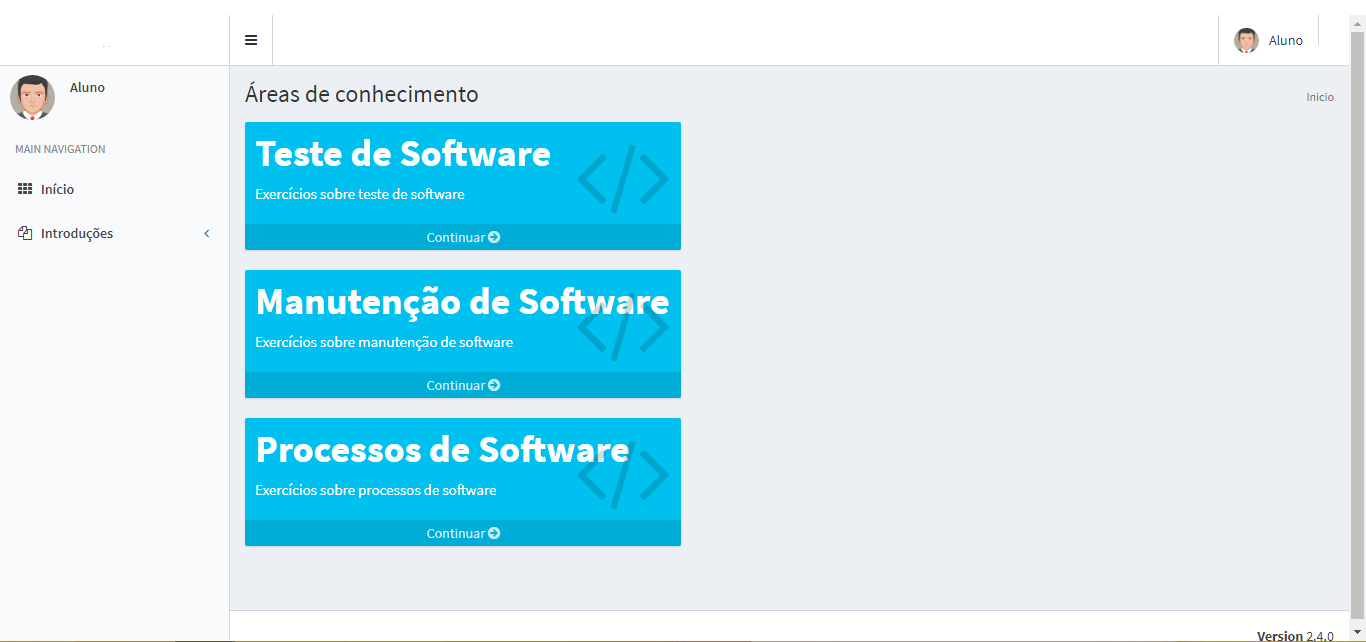
\includegraphics[width=1\textwidth]{./dados/figuras/areasTela}
    \fonte{Autoria Própria}
    \label{fig:figura-areas-telas}
\end{figure}

\begin{figure}[!htb]
    \centering
    \caption{Fases sobre teste de \textit{software}}
    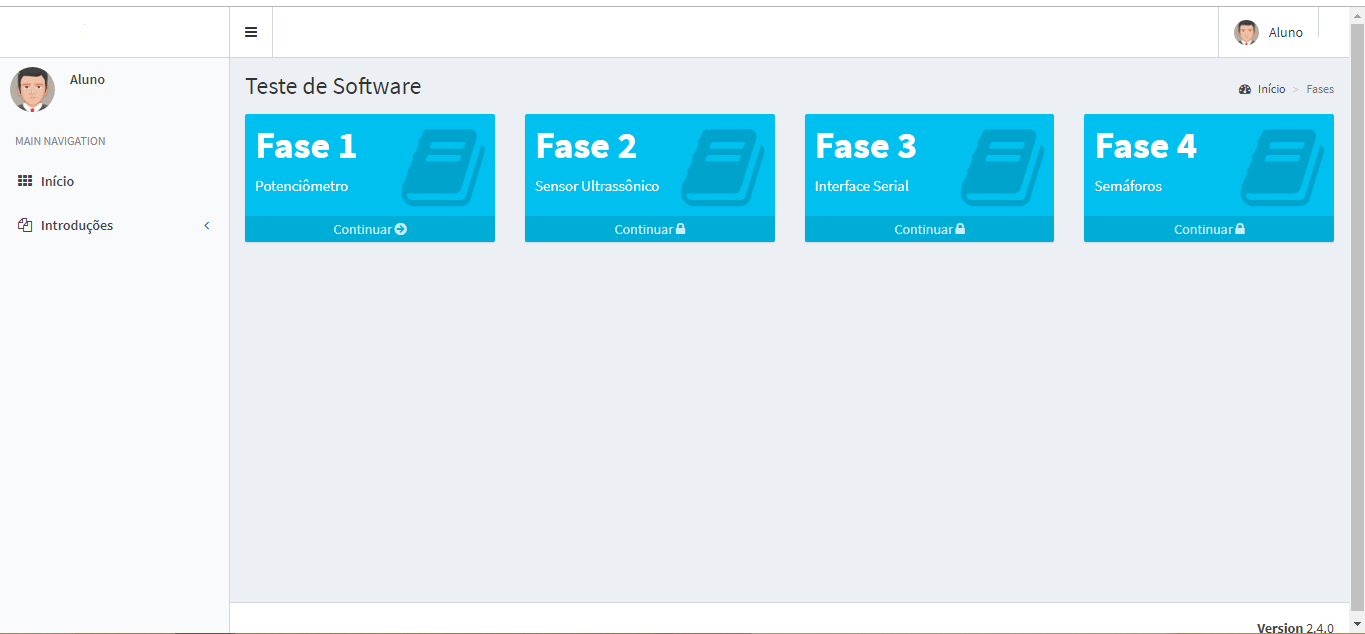
\includegraphics[width=1\textwidth]{./dados/figuras/fasesTela}
    \fonte{Autoria Própria}
    \label{fig:figura-fases-telas}
\end{figure}
 
Em cada fase será apresentado qual o objetivo, uma breve descrição, quais itens e componentes serão necessários, uma imagem do esquemático do projeto para montagem do circuito, um diagrama de classe dos itens utilizados, um diagrama de casos de uso, um diagrama de atividade, um diagrama de máquina de estado do projeto e um \textit{sketch}. Com essas informações o aluno deverá reconstruir o cenário proposto e realizar a atividade, que poderá surtir efeitos no \textit{sketch}, esquemático e diagramas. A Figura \ref{fig:figura-fase-tela} ilustra um exemplo de tela de uma das fases. Nela, o aluno realiza a leitura das atividades e tem acesso ao \textit{sketch}, esquemático e diagramas, para o auxílio na montagem do projeto. 
\begin{figure}[!htb]
    \centering
    \caption{Fase 1 - teste de \textit{software}}
    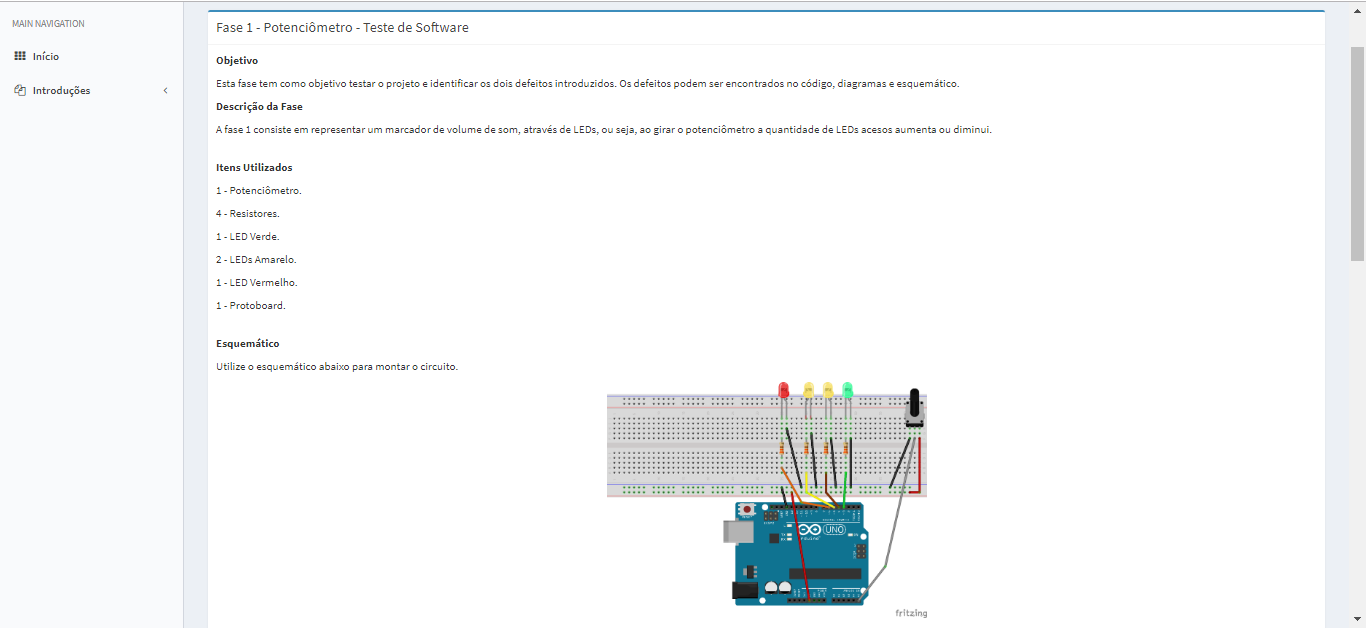
\includegraphics[width=1\textwidth]{./dados/figuras/faseTela}
    \fonte{Autoria Própria}
    \label{fig:figura-fase-tela}
\end{figure}

\section{FERRAMENTAS}
\label{sec:ferramentas}

\section{EXECUÇÃO DA APLICAÇÃO E ANÁLISE DE RESULTADOS}
\label{sec:execAppAnaliseResultados}
Para a avaliação da aceitação, motivação, engajamento, consolidação e aquisição de conhecimento causado pelo artefato gerado neste trabalho, o mesmo será utilizado por alunos da disciplina Engenharia de \textit{Software}, que possuem um conhecimento prévio sobre linguagem de programação, orientação a objetos, circuitos eletrônicos e alguns conceitos nos temas abordados neste trabalho. Ao término da utilização, os alunos darão um \textit{feedback} através de um questionário baseado na escala \texttt{likert}, um tipo de escala psicométrica comumente utilizada em pesquisas de opinião, onde a cada afirmação o pesquisado deve escolher um valor de 1 a 5. O valor um retrata o total desacordo ou negação, e o valor cinco representa o total acordo ou aceitação.


\chapter{CRONOGRAMA}
\label{chap:cronograma}
A figura \ref{fig:figura-cronograma} apresenta o cronograma as atividades previstas para este trabalho, sendo distribuídas entre Agosto de 2018 a Junho de 2019.

\begin{figure}[!htb]
    \centering
    \caption{Cronograma}
    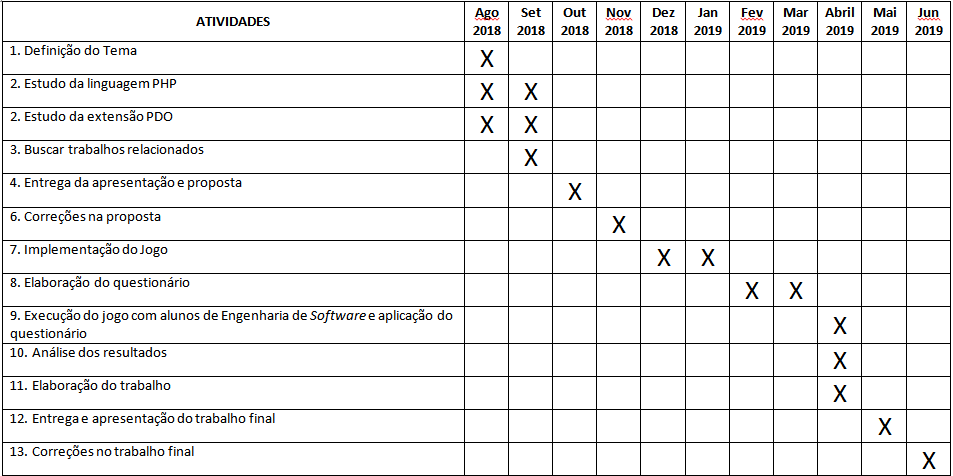
\includegraphics[width=1\textwidth]{./dados/figuras/cronogramaTCC}
    \fonte{Autoria Própria}
    \label{fig:figura-cronograma}
\end{figure}